\documentclass[11pt,a4paper]{ctexart}
\usepackage[a4paper,margin=2.2cm]{geometry}
\usepackage{graphicx}
\usepackage{booktabs}
\usepackage{float}
\usepackage{longtable}
\usepackage{array}
\usepackage{caption}
\usepackage{subcaption}
\usepackage{hyperref}
\usepackage{xcolor}
\usepackage{enumitem}
\usepackage{setspace}
\usepackage{titlesec}

\setstretch{1.25}
\hypersetup{colorlinks=true,linkcolor=blue,urlcolor=blue}
\titleformat{\section}{\Large\bfseries}{\thesection}{0.8em}{}
\titleformat{\subsection}{\large\bfseries}{\thesubsection}{0.8em}{}

\title{\textbf{给非本领域读者看的完整项目报告\\可解释药物脂溶性预测平台}}
\author{QSAR / XAI / 平台化项目说明}
\date{2026-03-15}

\begin{document}
\maketitle
\tableofcontents
\newpage

\section{项目一句话总结}
本项目的目标是：\textbf{根据分子结构预测脂溶性，并把结果做成可解释、可验证、可在线访问的网页与 API 工具。}

如果把它说得更口语一些，它就是一个“药物分子实验前预筛选助手”：输入一个分子的 \texttt{SMILES}，平台输出该分子的脂溶性预测值，并解释模型为什么这么判断。

\section{为什么要做这个项目}
脂溶性（lipophilicity）是药物研发中的关键性质，它影响吸收、分布、膜通透性和成药性。实验测量可靠，但耗时耗力，因此在实验前先用计算方法做预筛选非常有价值。

\begin{figure}[H]
    \centering
    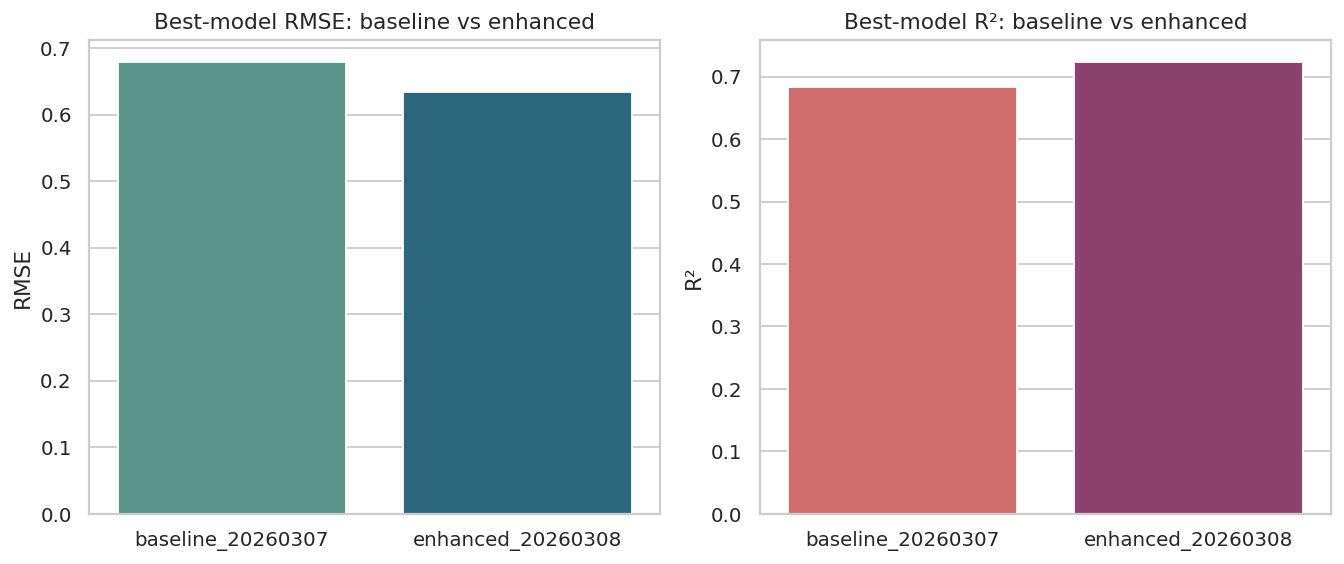
\includegraphics[width=0.9\textwidth]{../figures/14_baseline_vs_enhanced.png}
    \caption{增强版模型相对于基线模型的效果提升}
\end{figure}

\section{完整工作流}
本项目可以概括为 8 个步骤：
\begin{enumerate}[leftmargin=2em]
    \item 确定研究问题：预测药物脂溶性；
    \item 获取并清洗真实公开数据；
    \item 将分子结构转成机器可读特征；
    \item 建立基线模型；
    \item 做增强模型与集成学习；
    \item 做更严格的 scaffold 验证；
    \item 做 SHAP / XAI 可解释性分析；
    \item 做成在线平台和 API。
\end{enumerate}

\section{数据从哪里来}
项目使用公开的 Lipophilicity 数据集，清洗后保留 4200 个分子。每个分子带有真实实验测得的脂溶性标签，因此项目不是基于模拟数据，而是基于真实公开数据。

\section{模型怎么理解分子}
项目用了三类结构表示：
\begin{itemize}[leftmargin=2em]
    \item RDKit 理化描述符；
    \item Morgan Fingerprints；
    \item MACCS Keys。
\end{itemize}
这样既保留了药学上容易理解的整体性质，也保留了具体结构片段的信息。

\section{模型结果怎么理解}
增强版最佳模型是 \texttt{Weighted\_Ensemble\_rich}，在随机划分测试集上取得：
\begin{itemize}[leftmargin=2em]
    \item $R^2 = 0.7232$
    \item $RMSE = 0.6346$
    \item $MAE = 0.4517$
\end{itemize}

严格验证下，最佳模型 \texttt{Weighted\_Ensemble\_scaffold} 取得：
\begin{itemize}[leftmargin=2em]
    \item Mean $R^2 = 0.7138 \pm 0.0215$
    \item Mean $RMSE = 0.6489 \pm 0.0296$
\end{itemize}

\begin{figure}[H]
    \centering
    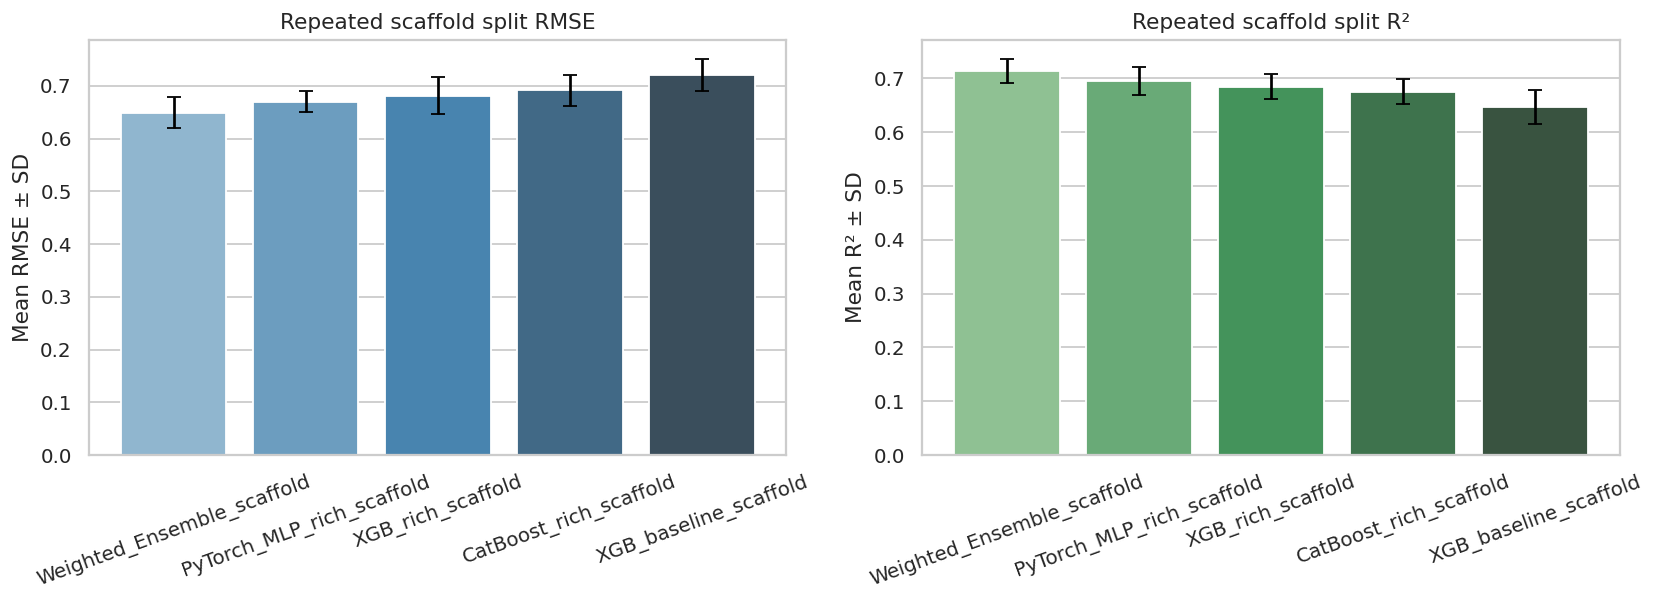
\includegraphics[width=0.9\textwidth]{../figures/16_scaffold_repeat_summary.png}
    \caption{Repeated scaffold split 严格验证结果}
\end{figure}

\section{为什么说它不是黑盒}
项目使用 SHAP 解释模型，说明模型整体最关注哪些特征，以及某个具体分子为什么会被预测成高脂溶性或低脂溶性。

在全局解释中，重要特征包括：\texttt{MolLogP}、\texttt{fr\_COO}、\texttt{VSA\_EState5}、\texttt{MACCS\_104} 等，这些都与药学常识具有明确对应关系。

\begin{figure}[H]
    \centering
    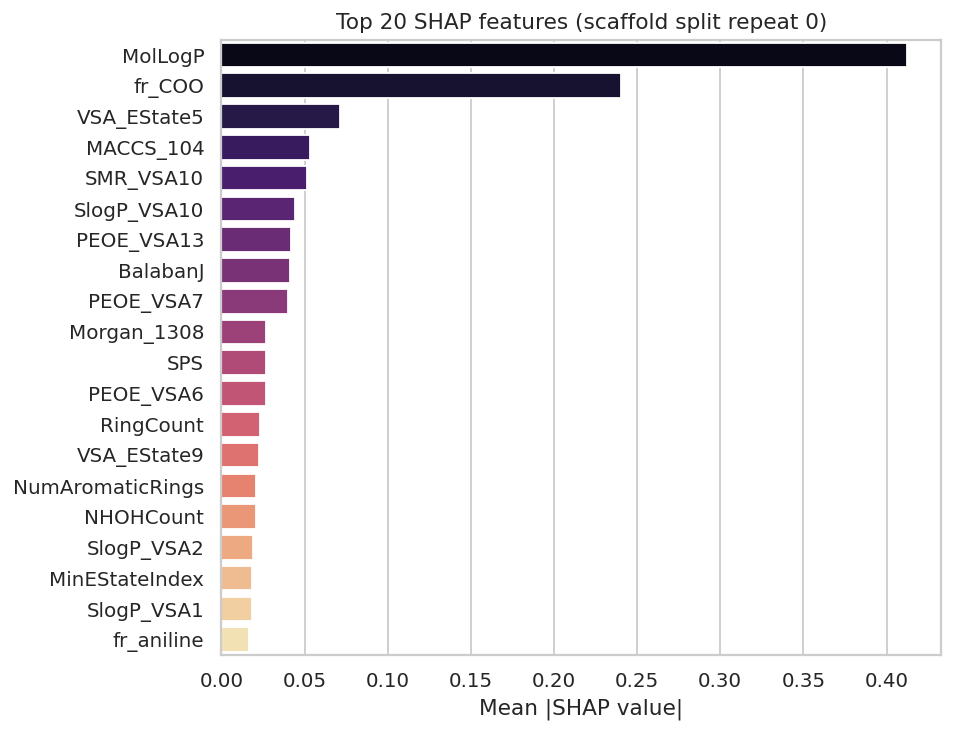
\includegraphics[width=0.82\textwidth]{../figures/19_shap_top20_bar.png}
    \caption{SHAP 全局重要特征图}
\end{figure}

\begin{figure}[H]
    \centering
    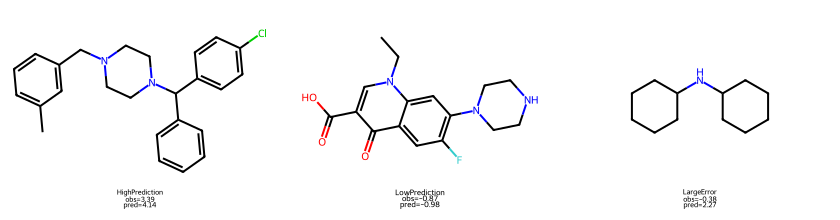
\includegraphics[width=0.82\textwidth]{../figures/22_shap_case_molecules.png}
    \caption{局部解释代表性分子案例}
\end{figure}

\section{平台做成了什么样}
项目进一步做成了可访问的网页平台与 JSON API。这样别人不需要读代码，也可以直接输入一个分子结构并获得预测与解释。

平台具备：
\begin{itemize}[leftmargin=2em]
    \item 单分子预测；
    \item 结果图展示；
    \item 严格验证结果展示；
    \item SHAP 解释展示；
    \item Gemini 辅助说明（可选）。
\end{itemize}

\section{这个项目最有价值的地方}
这个项目的价值不只是“预测一个数字”，而是同时具备：
\begin{itemize}[leftmargin=2em]
    \item 真实公开数据；
    \item 结构增强建模；
    \item 严格验证；
    \item SHAP 可解释性；
    \item 网页平台与 API；
    \item Gemini 辅助解释层。
\end{itemize}

因此，它不是一个简单的课程作业，而是一个更接近真实科研和真实应用场景的小型计算药学工具。

\section{读者最容易问的几个问题}
\subsection*{问题 1：为什么选脂溶性？}
因为脂溶性直接影响药物吸收、分布和膜通透性，是非常核心的药学性质。

\subsection*{问题 2：为什么还要做 scaffold 验证？}
因为随机划分容易偏乐观，scaffold 验证更接近“面对新骨架分子”的真实场景。

\subsection*{问题 3：SHAP 能证明什么？}
SHAP 不能证明因果，但能说明模型主要在依据哪些有化学意义的特征进行判断。

\subsection*{问题 4：Gemini 在这里做什么？}
Gemini 不负责核心预测，而是把已有模型结果翻译成更适合药学展示和答辩表达的自然语言说明。

\section{结论}
这个项目把真实公开数据、分子特征工程、机器学习、深度学习、严格验证、可解释性和在线平台结合起来，形成了一个完整、可讲、可展示、可部署的跨学科作品。

\end{document}
